\documentclass{beamer}
%\usetheme{Warsaw}
\usetheme{AnnArbor}
\defbeamertemplate*{footline}{shadow theme}
{% this section is for frame numbering
  \leavevmode%
  \hbox{\begin{beamercolorbox}[wd=.5\paperwidth,ht=2.5ex,dp=1.125ex,leftskip=0.3cm plus1fil,rightskip=0.3cm]{author in head/foot}%
    \usebeamerfont{author in head/foot}\hfill\insertshortauthor
  \end{beamercolorbox}%
  \begin{beamercolorbox}[wd=.5\paperwidth,ht=2.5ex,dp=1.125ex,leftskip=.3cm,rightskip=.3cm plus1fil]{title in head/foot}%
    \usebeamerfont{title in head/foot}\insertshorttitle\hfill\insertframenumber\,/\,\inserttotalframenumber
  \end{beamercolorbox}}%
  \vskip0pt%
}

\usecolortheme{spruce}
\usepackage[english]{babel}
\usepackage[utf8]{inputenc}
\usepackage{graphicx}
\usepackage[absolute,overlay]{textpos}% pour la fonction textblock
\usepackage{tikz} % pour rendre figures transparentes
\setbeamertemplate{frame numbering}[fraction]
\usepackage{listings}
\usepackage{color}
\usepackage{amsmath,amssymb,mathrsfs,amsthm}
\definecolor{gray}{rgb}{0.92,0.92,0.92}
\lstset{frame=tb,
	backgroundcolor=\color{gray},
	language=R,
	aboveskip=3mm,
	belowskip=3mm,
	showstringspaces=false,
	columns=flexible,
	basicstyle={\small\ttfamily},
	numbers=none,
	breaklines=true,
	breakatwhitespace=true,
	tabsize=3
}
\beamertemplatenavigationsymbolsempty % Remove bar 
\newcommand{\Ctreize}{$\delta$\textsuperscript{13}C\xspace}

\newcommand{\Odixhuit}{$\delta$\textsuperscript{18}O\xspace}
\beamersetuncovermixins{\opaqueness<1>{25}}{\opaqueness<2->{15}}
\begin{document}
	
\newcommand{\un}{\textunderscore}

%slide 1 (Title)
%%%%%%%%%%%%%%%%%%%%%%%%%%%%%%%%%%%%%%%%%%%%%%%%
\title[Projet de thèse de doctorat]{Modélisation des effets du climat et de la génétique sur les propriétés du bois} 
%\subtitle{projet}
\author{\textbf{André SORO}}
\date{}
\institute{19 Avril 2018}

\begin{textblock*}{11cm}(0.9cm,0.5cm)
	
\includegraphics[height = 0.9cm]{logo-universite-laval}
	\hfill
	
\includegraphics[height = 1.1cm]{logo_crmr}
\end{textblock*}


\begin{textblock*}{5cm}(0.85cm,7.5cm)
	\underline{Directeur}\\
	Alexis ACHIM\\
\end{textblock*}
	
	
\begin{textblock*}{5cm}(7cm,7.07cm)
	\begin{flushright}
		\underline{Co-directeur}\\
	    Patrick LENZ\\
	\end{flushright}
\end{textblock*}

%slide
%%%%%%%%%%%%%%%%%%%%%%%%%%%%%%%%%%%%%%%%%%%%%%%%
\usebackgroundtemplate{%
	\tikz\node[opacity=0.35] {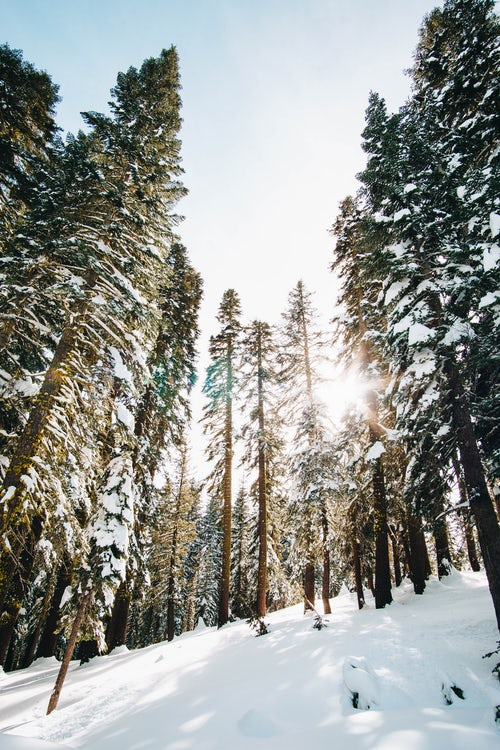
\includegraphics[height={\paperheight} ,width=\paperwidth]{foret1}};}
\begin{frame}
	\titlepage
\end{frame}	

\usebackgroundtemplate{} % fond blanc à partir d'ici


%slide
%%%%%%%%%%%%%%%%%%%%%%%%%%%%%%%%%%%%%%%%%%%%%%%%

\section{Introduction}
\begin{frame}{Importance de l'épinette blanche}
	
\begin{columns}
	
	\begin{column}{0.45\textwidth}
		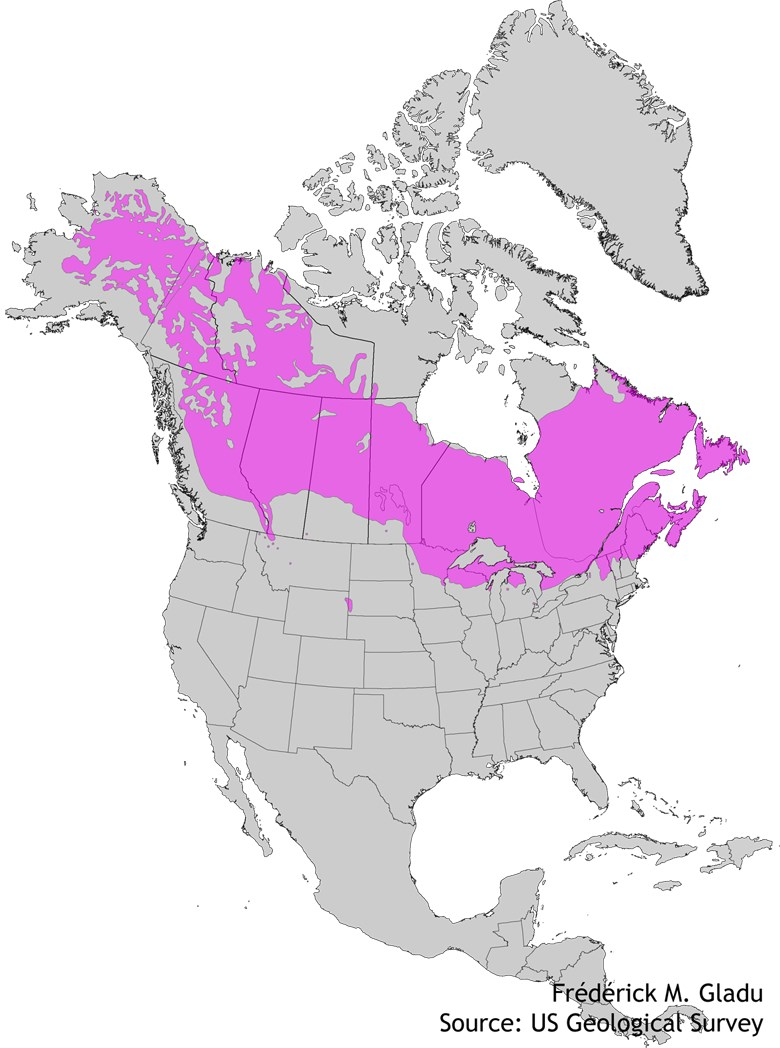
\includegraphics[width=\textwidth]{distribution.jpg}
	\end{column}
	
	\begin{column}{0.4\textwidth}
		\begin{itemize} 
			\item Grande répartition  \\
			\vspace{0.5cm}
			\item Forte plasticité\\
			\vspace{0.5cm}
			\item L'épinette blanche est fortement reboisée (15-20 millions au Qc)
		\end{itemize}	
	\end{column}
	
\end{columns}

\end{frame}

%slide
%%%%%%%%%%%%%%%%%%%%%%%%%%%%%%%%%%%%%%%%%%%%%%%%
\begin{frame}{Contrôle génétique des propriétés du bois}
	
	\begin{columns}
		
		\begin{column}{0.5\textwidth}
			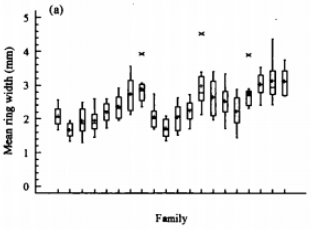
\includegraphics[width=\textwidth]{controlgeneMosedale1996}
		\end{column}
		
		\begin{column}{0.5\textwidth}
			\begin{itemize} 
				\item La famille affecte la largeur des cernes\\
				\vspace{0.5cm}
				\item La génétique influence les propriétés du bois comme la densité (Lenz et al. 2010)\\
			\end{itemize}	
		\end{column}
		
	\end{columns}
		
	\begin{textblock*}{10cm}(2cm,7.5cm)
		\tiny Mosedale et al. (1996)
	\end{textblock*}
\end{frame}

%slide
%%%%%%%%%%%%%%%%%%%%%%%%%%%%%%%%%%%%%%%%%%%%%%%%
\begin{frame}{Relation activité cambiale-climat}
	\begin{columns}
		
		\begin{column}{0.6\textwidth}
			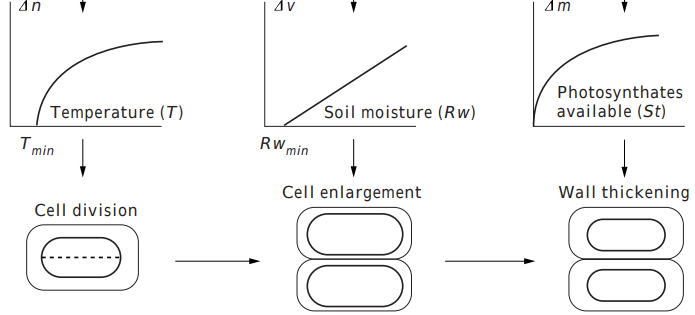
\includegraphics[width=\textwidth]{cambimDeluze1998}
		\end{column}
		
		\begin{column}{0.4\textwidth}
			\begin{itemize} 
				\item L'environnement influence l'activité cambiale\\
				\vspace{0.5cm}
				\item Le climat influence la croissance radiale de l'arbre\\
			\end{itemize}	
		\end{column}
		
	\end{columns}
	
	\begin{textblock*}{10cm}(2cm,8.5cm)
		\tiny Deleuze et Houllier (1998)
	\end{textblock*}
\end{frame}

%slide
%%%%%%%%%%%%%%%%%%%%%%%%%%%%%%%%%%%%%%%%%%%%%%%%
\begin{frame}{Signature isotopique}
	\begin{columns}
		
		\begin{column}{0.4\textwidth}
			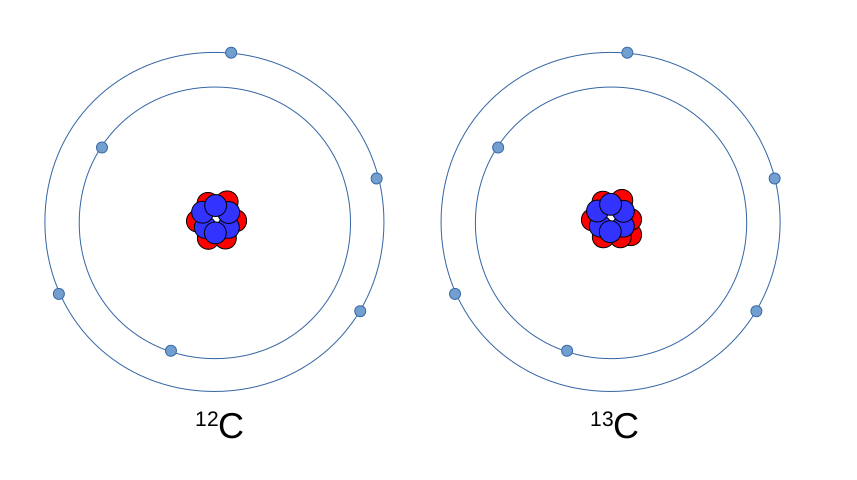
\includegraphics[width=\textwidth]{Isotope}
		\end{column}
		
		\begin{column}{0.6\textwidth}
			\begin{itemize} 
				\item Estimation de l'impact du climat sur le bois\\
				\vspace{0.5cm}
				\item Pourquoi la signature isotopique?\\
			\end{itemize}	
		\end{column}
		
	\end{columns}
			\begin{textblock*}{10cm}(1cm,6.5cm)
				\tiny Isotopes de carbone
			\end{textblock*}

\end{frame}

%slide
%%%%%%%%%%%%%%%%%%%%%%%%%%%%%%%%%%%%%%%%%%%%%%%%
\begin{frame}{Relation climat-proportion d'isotopes stables}
	
\begin{columns}
	
	\begin{column}{0.6\textwidth}
		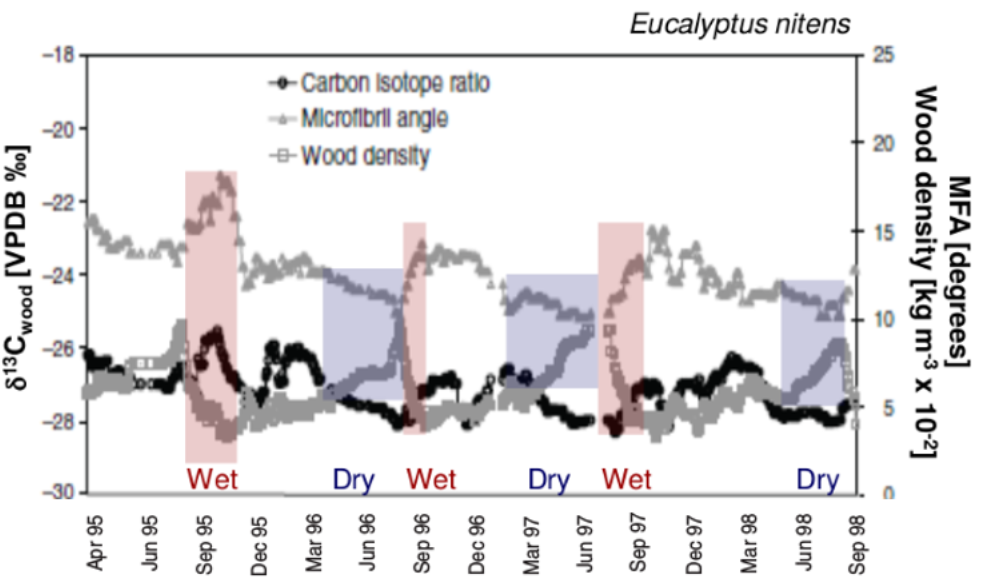
\includegraphics[width=\textwidth]{ctreizeDrew2009}
	\end{column}
		
	\begin{column}{0.4\textwidth}
		\begin{itemize} 
			\item Impact de la sécheresse sur la densité et l'AMF\\
			\vspace{0.5cm}
			\item Variation de la signature isotopique et des propriétés du bois\\
		\end{itemize}		
	\end{column}

\end{columns}
	\begin{textblock*}{10cm}(2cm,7.7cm)
		\tiny Drew et al. (2009)	
	\end{textblock*}
	
\end{frame}

%slide
%%%%%%%%%%%%%%%%%%%%%%%%%%%%%%%%%%%%%%%%%%%%%%%%


\begin{frame}{Objectifs}
	%\begin{textblock*}{12.5cm}(0.1cm,1.5cm)
		\begin{enumerate}[<+- | alert@+>]
		\item Identifier les familles/arbres aux profils de densité et largeur des cernes les plus uniformes\\
		\vspace{0.25cm}
	              $\Rightarrow$ Sélection pour reboisement\\
		\vspace{1cm}
		
		\item Evaluer l'influence de différents niveaux de sécheresse sur les propriétés du bois\\
		\vspace{0.25cm}
	        	$\Rightarrow$ Anticiper l'effet des changements climatiques\\
		\vspace{1cm}
		
		\item Analyser l'effet du climat et de la génétique sur $\delta$\textsuperscript{13}C, $\delta$\textsuperscript{18}O et les propriétés du bois\\
		\vspace{0.25cm}
		$\Rightarrow$ Comprendre la variation isotopique liée à la génétique\\
	    \end{enumerate}
	%\end{textblock*}
\end{frame}

%slide
%%%%%%%%%%%%%%%%%%%%%%%%%%%%%%%%%%%%%%%%%%%%%%%%
\section{Chapitre 1 : Caractérisation des profils uniformes}
\begin{frame}%{Chapitre 1}
\Large	\textbf{Chapitre 1} : Caractérisation des profils de densité et de la largeur des cernes et identification des familles avec le bois le plus uniforme face aux variations climatiques\\
	
\end{frame}
%slide
%%%%%%%%%%%%%%%%%%%%%%%%%%%%%%%%%%%%%%%%%%%%%%%%
\begin{frame}{Hypothèse}
	\begin{columns}
		
		\begin{column}{0.45\textwidth}
			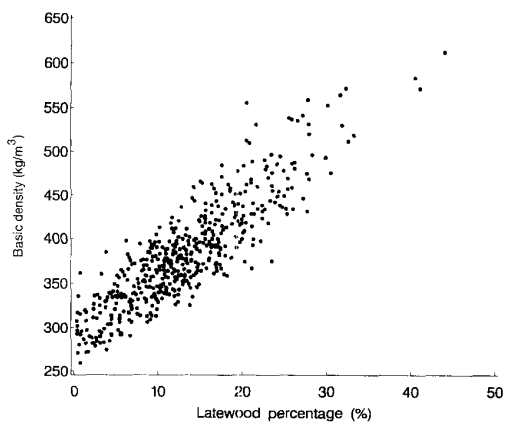
\includegraphics[width=\textwidth]{densityvsladewoodLindstrom1996}\\
		%	\vspace{0.7cm}
			%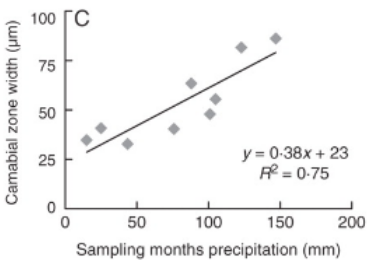
\includegraphics[width=\textwidth]{cambimDie2012}\\
		\end{column}
		
		\begin{column}{0.52\textwidth}
			\begin{itemize} 
				\item La densité du bois est fonction du pourcentage du bois final\\
				\vspace{0.5cm}
				\item Le climat influence l'activité cambiale (cf slide 6)\\
				\vspace{1cm} 
				$\Rightarrow$ Une sécheresse lors de la formation du bois final entraîne une baisse de densité
			\end{itemize}		
		\end{column}
		
	\end{columns}
 
	\begin{textblock*}{6cm}(0.01cm,8.2cm)	
	\tiny Lindstrom et al. (1996)
	\end{textblock*}
\end{frame}

%slide
%%%%%%%%%%%%%%%%%%%%%%%%%%%%%%%%%%%%%%%%%%%%%%%%
\begin{frame}{Hypothèse}
	
\Large \textbf{Hypothèse} : L’impact d’une sécheresse sur la densité du bois dépend du moment où elle survient lors de la saison de végétation.
	
\end{frame}

%slide
%%%%%%%%%%%%%%%%%%%%%%%%%%%%%%%%%%%%%%%%%%%%%%%%

\begin{frame}{Plan de l'expérience}
	
		%\centering
		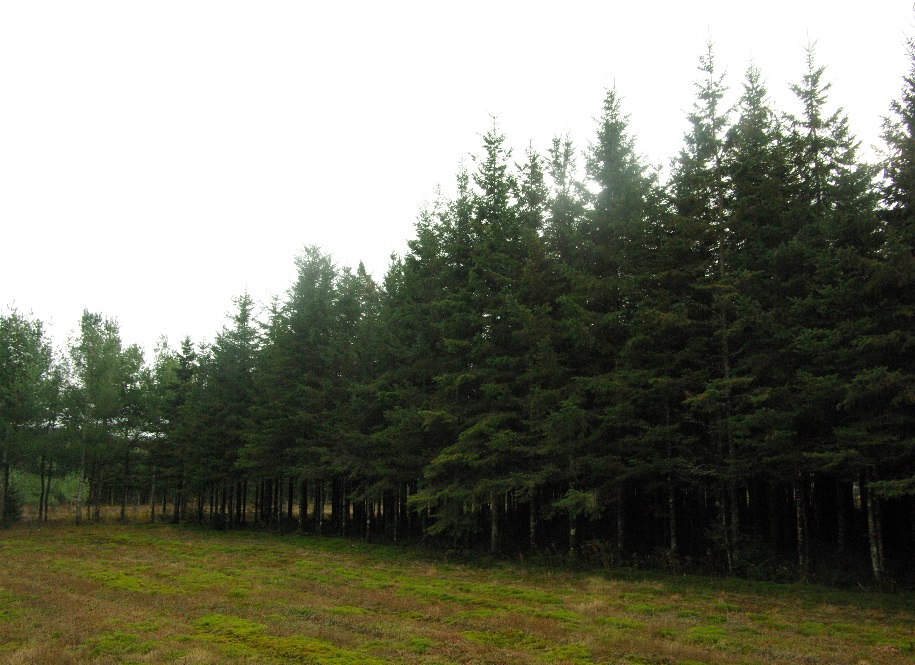
\includegraphics[height=5.7cm, width=7cm]{Site_etude}
	\begin{textblock*}{9.8cm}(7.1cm,3cm)
		\begin{itemize} %[<+- | alert@+>]
			\item Essais mis en place en 1999 \\
			\vspace{0.5cm}
			\item 2 sites : St-Casimir (Portneuf)\\
			et Asselin (Témiscouata)\\
			\vspace{0.5cm}
			\item 93 familles biparentales,\\
			 2500 individus \\
			%\vspace{0.5cm}
			%\item Effet du climat sur $\delta$\textsuperscript{13}C et $\delta$\textsuperscript{18} du bois
		\end{itemize}           
	\end{textblock*}
\end{frame}

%slide
%%%%%%%%%%%%%%%%%%%%%%%%%%%%%%%%%%%%%%%%%%%%%%%%

\begin{frame}{Méthodes et analyses statistiques}
	
\begin{textblock*}{12cm}(0.1cm,2cm)
	\begin{itemize} %[<+- | alert@+>]
		\item \textbf{Climat} : Par BioSim \\
		\vspace{0.5cm}
		\item \textbf{Densité} : Par densitométrie à rayons-X  \\
		\vspace{0.5cm}
		\item \textbf{Statistiques} : Modèles mixtes avec les variables suivantes\\
		\vspace{0.2cm}
		Dépendantes : la densité et la largeur des cernes\\
		\vspace{0.2cm}
		Fixes : les précipitations et les indices de sécheresse \\
		\vspace{0.2cm}
        Aléatoires : site, bloc, arbre et les croisements
		
	\end{itemize}
\end{textblock*}
	
\end{frame}
%slide
%%%%%%%%%%%%%%%%%%%%%%%%%%%%%%%%%%%%%%%%%%%%%%%%

\begin{frame}{Résultats attendus et conclusion}
	
	\begin{textblock*}{12cm}(0.1cm,3cm)
		\begin{itemize} %[<+- | alert@+>]
			\item Individus/familles aux profils uniformes \\
			\vspace{0.7cm}
			\item Sélection pour amélioration génétique  \\
			\vspace{0.7cm}
			\item Productivité et qualité de bois malgré les variations climatiques\\
		\end{itemize}
	\end{textblock*}
	
\end{frame}

%slide
%%%%%%%%%%%%%%%%%%%%%%%%%%%%%%%%%%%%%%%%%%%%%%%%
\section{Chapitre 2 : Sécheresse intense et propriétés du bois}
\begin{frame}%{Chapitre 2}
\Large	\textbf{Chapitre 2} : Modélisation de l’impact de différents niveaux de sécheresse sur les propriétés du bois et identification des clones peu sensibles\\
	
\end{frame}
%slide
%%%%%%%%%%%%%%%%%%%%%%%%%%%%%%%%%%%%%%%%%%%%%%%%
\begin{frame}{Hypothèse}
\begin{textblock*}{12cm}(0.1cm,3cm)
	\begin{itemize} %[<+- | alert@+>]
		\item AMF sensible aux variations climatiques (Xu et al. 2012)\\
		\vspace{0.7cm}
		\item La sécheresse intense entraîne une diminution de l'AMF (Wimmer et al. 2002)\\
		\vspace{0.7cm}
		\item Impact de la sécheresse sur la conductivité (Irvine et al. 1997)\\
	\end{itemize}
\end{textblock*}
\end{frame}

%slide
%%%%%%%%%%%%%%%%%%%%%%%%%%%%%%%%%%%%%%%%%%%%%%%%
\begin{frame}{Hypothèse}
	
\Large	\textbf{Hypothèse} : Le stress hydrique entraîne une diminution de l’angle des microfibrilles et affecte négativement la conductivité spécifique
	
\end{frame}

%slide
%%%%%%%%%%%%%%%%%%%%%%%%%%%%%%%%%%%%%%%%%%%%%%%%
\begin{frame}{Plan de l'expérience}
		\begin{columns}			
			\begin{column}{0.7\textwidth}
				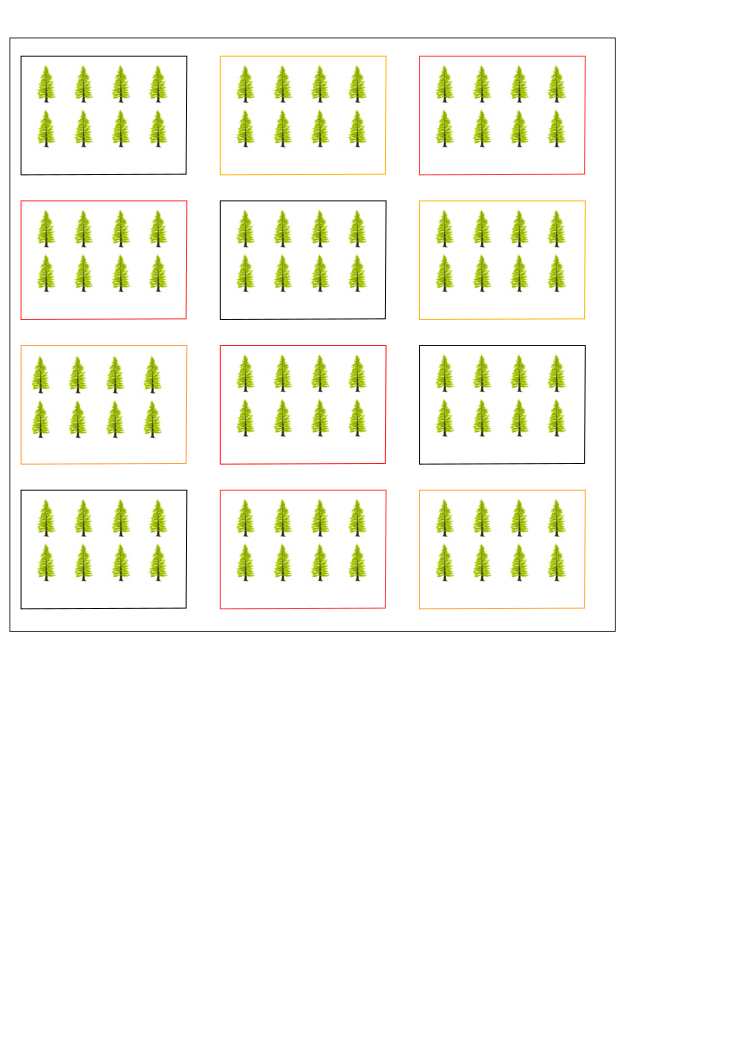
\includegraphics[width=\textwidth]{Plan_experimentation}\\
			\end{column}
			\begin{column}{0.3\textwidth}
					\begin{textblock*}{10cm}(7.7cm,3cm)
				\begin{itemize} 
                	\item 3 traitements\\
                	\vspace{0.2cm}			
					\item 420 plants\\
					\vspace{0.2cm}
				    \item 12 Blocs \\
					\vspace{0.2cm} 
					\item 35 plants/bloc \\
					\vspace{0.2cm}
					\item 1 plant de chaque \\
					clone/bloc \\
				\end{itemize}
					\end{textblock*}		
			\end{column}
			
		\end{columns}
	
\end{frame}
%slide
%%%%%%%%%%%%%%%%%%%%%%%%%%%%%%%%%%%%%%%%%%%%%%%%

\begin{frame}{Méthodes}
	
	\begin{textblock*}{11cm}(0.1cm,2.7cm)
		\begin{itemize} %[<+- | alert@+>]
			\item \textbf{AMF} : par diffractomètre à rayon-X (2mm de résolution) \\
			\vspace{1cm}
			\item \textbf{Masse volumique} : à partir des mesures anatomiques
			%\begin{equation}\label{eq:1}
			%\rho_{tracheide} = \rho_{paroi}\cdot\frac{A_{paroi}}{A_{tracheide}}
			%\end{equation}\\ 
			\vspace{1cm}
			\item \textbf{Conductivité spécifique} : à partir des mesures anatomiques
			%\begin{equation}\label{eq:2}
		%	k_{s} = N\cdot \frac{\pi \cdot \rho_{w}}{128 \cdot \eta} \cdot <L>^{4}
			%\end{equation}\\
			
			
		\end{itemize}
	\end{textblock*}
	
\end{frame}
%slide
%%%%%%%%%%%%%%%%%%%%%%%%%%%%%%%%%%%%%%%%%%%%%%%%

\begin{frame}{Analyses statistiques}
	
	\begin{textblock*}{12cm}(0.1cm,2.9cm)
		Modèles mixtes avec les variables suivantes\\
		
		\begin{itemize} %[<+- | alert@+>]
			\item \textbf{Dépendantes} : la densité, l’angle des microfibrilles et la conductivité spécifique \\
			\vspace{0.5cm}
			\item \textbf{Fixes} : les trois niveaux de traitements et le clone\\
			\vspace{0.5cm}
			\item \textbf{Aléatoire} : bloc\\			
		\end{itemize}
	\end{textblock*}
	
\end{frame}
%slide
%%%%%%%%%%%%%%%%%%%%%%%%%%%%%%%%%%%%%%%%%%%%%%%%

\begin{frame}{Résultats attendus et conclusion}
	
	\begin{textblock*}{10cm}(0.1cm,3cm)
		\begin{itemize} %[<+- | alert@+>]
			\item Réaction (AMF, densité etc) différente entre traitements \\
			\vspace{0.7cm}
			\item Stratégie d'adaptation différente entre différents clones  \\
			\vspace{0.7cm}
			\item Relation entre conductivité et propriétés du bois\\
			\vspace{0.7cm}
			\item Conséquence de la stratégie\\
		\end{itemize}
	\end{textblock*}
	
\end{frame}
%slide
%%%%%%%%%%%%%%%%%%%%%%%%%%%%%%%%%%%%%%%%%%%%%%%%
\section{Chapitre 3 : Effets du climat sur $\delta$\textsuperscript{13}C et $\delta$\textsuperscript{18}O}
\begin{frame}%{Chapitre 3}
\Large	\textbf{Chapitre 3} : Quantification des effets du climat	sur la variation de la proportion d’isotopes stables ($\delta$\textsuperscript{13}C et $\delta$\textsuperscript{18}O) en lien avec les familles\\
	
\end{frame}

%slide
%%%%%%%%%%%%%%%%%%%%%%%%%%%%%%%%%%%%%%%%%%%%%%%%
\begin{frame}{Hypothèse}
	\begin{columns}			
		\begin{column}{0.47\textwidth}
			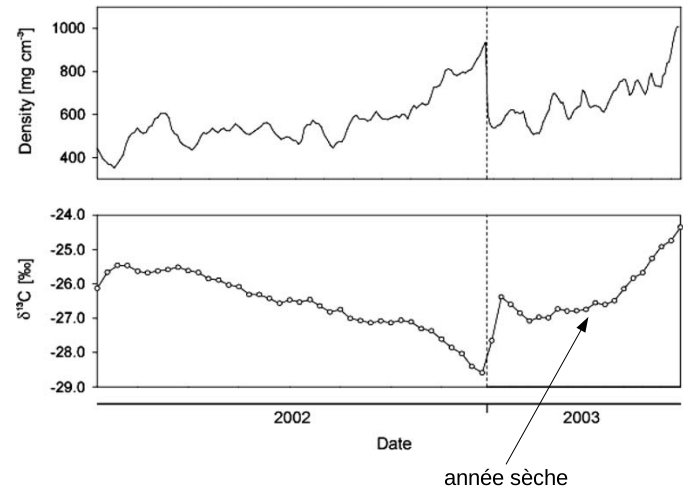
\includegraphics[width=\textwidth]{CtreizeSkomarkova2006}\\
		\end{column}
		\begin{column}{0.4\textwidth}
			\begin{textblock*}{6cm}(6.3cm,3cm)
				\begin{itemize} 
					\item La sécheresse affecte la signature isotopique et la densité\\
					\vspace{0.2cm}
					\item Augmentation de la signature isotopique pendant la sécheresse\\
	     	\end{itemize}
			\end{textblock*}		
		\end{column}
		
	\end{columns}
	\begin{textblock*}{8cm}(4.3cm,2.7cm)
		\tiny Fagus sylvatica
	\end{textblock*}
	\begin{textblock*}{8cm}(0.1cm,7.3cm)
		\tiny Skomarkova et al. (2006)
	\end{textblock*}
\end{frame}

%slide
%%%%%%%%%%%%%%%%%%%%%%%%%%%%%%%%%%%%%%%%%%%%%%%%
\begin{frame}{Hypothèse}
	
\Large	\textbf{Hypothèse} : Une part significative de variabilité de la relation entre $\delta$\textsuperscript{13}C et $\delta$\textsuperscript{18}O du bois et les conditions météorologiques est associée à la différence génétique.
	
\end{frame}

%slide
%%%%%%%%%%%%%%%%%%%%%%%%%%%%%%%%%%%%%%%%%%%%%%%%
\begin{frame}{Matériel et site d'étude}
	
	\Large Site d'étude est le même que celui du chapitre 1 :\\
	
	St-Casimir et Asselin
	
\end{frame}

%slide
%%%%%%%%%%%%%%%%%%%%%%%%%%%%%%%%%%%%%%%%%%%%%%%%
\begin{frame}{Méthode}
	\begin{columns}			
		\begin{column}{0.5\textwidth}
			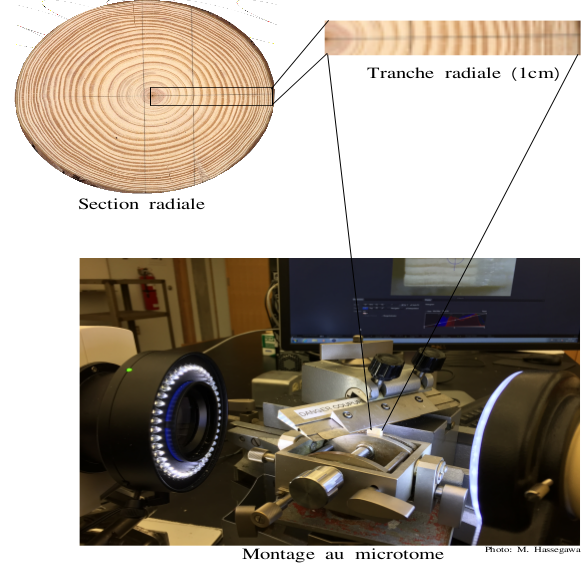
\includegraphics[width=\textwidth]{Mesure_sotopique.png}\\
		\end{column}
		\begin{column}{0.4\textwidth}
			\begin{textblock*}{6cm}(6.7cm,4.5cm)
				\begin{itemize} 
					\item Coupe anatomique\\
					%\vspace{0.2cm}
					%\item Microtome avec 2 caméras\\
					%\vspace{0.2cm}
					%\item Microtome à 20-30 microns\\
					\vspace{0.2cm}
					\item Extraction de la cellulose\\
				\end{itemize}
			\end{textblock*}		
		\end{column}
		
	\end{columns}
		
	\only<1>{\begin{textblock*}{9cm}(0.6cm,8.5cm)
			\tiny Préparation d'échantillons pour extraction de cellulose
		\end{textblock*}}
	
\end{frame}
%slide
%%%%%%%%%%%%%%%%%%%%%%%%%%%%%%%%%%%%%%%%%%%%%%%%

\begin{frame}{Analyses statistiques}
	
	\begin{textblock*}{12cm}(0.1cm,2.9cm)
		Modèles mixtes avec les variables suivantes\\
		
		\begin{itemize} %[<+- | alert@+>]
			\item \textbf{Dépendante} : la signature isotopique \\
			\vspace{0.5cm}
			\item \textbf{Fixes} : les précipitations, les indices de sécheresse et la famille\\
			\vspace{0.5cm}
			\item \textbf{Aléatoire} : le site, le bloc et l'arbre\\			
		\end{itemize}
	\end{textblock*}
	
\end{frame}
%slide
%%%%%%%%%%%%%%%%%%%%%%%%%%%%%%%%%%%%%%%%%%%%%%%%
\begin{frame}{Résultats attendus et conclusion}
	
	\begin{textblock*}{11cm}(0.1cm,3cm)
		\begin{itemize} %[<+- | alert@+>]
			\item Lien entre climat et signature isotopique \\
			\vspace{0.7cm}
			\item Variabilité de la signature isotopique associée à la génétique\\
			\vspace{0.7cm}
			\item Relation signature isotopique et propriétés du bois\\
		\end{itemize}
	\end{textblock*}
	
\end{frame}
%slide
%%%%%%%%%%%%%%%%%%%%%%%%%%%%%%%%%%%%%%%%%%%%%%%%
\section{Conclusion }
\begin{frame}{Conclusion générale}
	
	\begin{textblock*}{11cm}(0.1cm,3cm)
		\begin{itemize} %[<+- | alert@+>]
			\item Identifier les arbres/familles aux profils moins marqués par les variations du climat\\
			\vspace{0.7cm}
			\item Sélectionner des arbres pour l'amélioration génétique et le reboisement\\
			\vspace{0.7cm}
			\item Anticiper l'effet des changements climatiques sur la production et la qualité du bois\\
		\end{itemize}
	\end{textblock*}
	
\end{frame}
%slide
%%%%%%%%%%%%%%%%%%%%%%%%%%%%%%%%%%%%%%%%%%%%%%%%
\section{ }
\begin{frame}%{Résultats attendus et conclusion}
	
	\begin{textblock*}{10cm}(1.5cm,4.7cm)
		\centering
		{\Large \textbf{Merci de votre attention}}\\	
	\end{textblock*}
	
\end{frame}
%slide
%%%%%%%%%%%%%%%%%%%%%%%%%%%%%%%%%%%%%%%%%%%%%%%%
\begin{frame}{Calendrier prévisionnel de la thèse}
	
\includegraphics[width=\textwidth]{Calendrier.pdf}
	
\end{frame}
%slide
%%%%%%%%%%%%%%%%%%%%%%%%%%%%%%%%%%%%%%%%%%%%%%%%


\end{document}